The sPHENIX detector is a cylindrical detector covering
$\left|\eta\right| \leq 1.1$ and the full azimuth.  It is designed to use
the former BaBar superconducting solenoid to contain
an inner tracking system out to 80~cm in radius followed by an
electromagnetic calorimeter and the first of two longitudinal segments of
a hadronic calorimeter, which is not instrumented in the project baseline.  The second
longitudinal segment of the hadronic calorimeter, which is instrumented to
$|\eta| \leq 1.1$, also serves as
the magnet flux return, surrounding the magnet cryostat.


The primary components of the sPHENIX reference design are as follows.

\begin{description}

\item[Magnetic Solenoid]  Built for the BaBar experiment at
  SLAC, the magnet became available after the termination of the BaBar
  program.  The cryostat has an inner radius of 140~cm and is 33~cm
  thick, and can produce a central field of 1.4~T.

\item[Tracking system] The tracking system consist of three components:

\begin{description}

\item[Time Projection Chamber] A TPC with an outer radius of about 80~cm
measures space points of charged tracks, which provides momentum resolution that can
separate the Upsilon states in decays to $e^+e^-$.

\item[Intermediate Tracking] The Intermediate Tracker is a silicon strip
detector consisting of two layers which can measure space points
on charged tracks inside the inner radius of the TPC for robust tracking
even in a high multiplicity heavy ion collision with time resolution that
can separate pileup in the TPC.
This detector is based on commercial silicon
sensors read out with the FPHX ASIC developed for the PHENIX FVTX detector and
is a RIKEN and RIKEN-Brookhaven Research Center contribution to the sPHENIX
experiment.

\item[MAPS Vertex Detector] A Monolithic Active Pixel (MAPS) vertex
detector in close proximity to the beam pipe is to provide high precision
vertex measurements to determine displaced vertices from decays
of particles containing $b$ and $c$ quarks, and provide additional precisely
measured space points for charged particle tracking.  This detector is
proposed and developed as a separate upgrade to the sPHENIX proposal,
based on duplicating as much as possible the ALICE Inner Tracking System (ITS)
detector.

\end{description}

\item[Electromagnetic Calorimeter] Tungsten-scintillating fiber
  sampling calorimeter inside the magnet bore read out with silicon
  photo-multipliers.  The calorimeter has a small Moli\`ere radius and
  short radiation length, allowing for a compact design.

\item[Inner Hadronic Calorimeter] Sampling calorimeter of non-magnetic
  metal and scintillator located inside the magnet bore, which is not part of the
  DOE funded proposal, but which could be instrumented at a later time with 
  non-DOE funding.

\item[Outer Hadronic Calorimeter] Sampling calorimeter of magnet steel
  and scintillator located outside the cryostat, which doubles as the flux
  return for the solenoid.

\end{description}

In the following list we provide a high-level mapping between physics
aims and various detector requirements.  The justification for these
requirements is then discussed in more detail in subsequent sections.

\begin{description}

\item[Upsilons] The key to the physics is high statistics \pp, \pA,
  and \hic data sets, with mass resolution and signal-to-background
  sufficient to separate the three states of the $\Upsilon$ family.
  \begin{itemize}
  \item large geometric acceptance ($\Delta\phi = 2\pi$ and $|\eta| < 1.1$)
  \item high rate data acquisition (15~kHz)
  \item trigger for electrons from $\Upsilon\rightarrow\epem$ ($>90$\% efficiency)
    in \pp and \pA
  \item track reconstruction efficiency $>90$\% and purity $>90$\% for
    $\pT > 3$~GeV/c
  \item less than 125 MeV/$c^2$ mass resolution on Upsilon states.
  \item electron identification with efficiency $>70$\% and charged
    pion rejection of 90:1 or better in central \auau at $\pT =
    4$~GeV/c.
  \end{itemize}

  \hrule

\item[Jets] The key to the physics is to cover jet energies of
  20--70~GeV, for all centralities, for a range of jet sizes, with
  high statistics and performance insensitive to the details of jet
  fragmentation.

  \begin{itemize}
  \item energy resolution $<120\%/\sqrt{E_{\mathrm{jet}}}$ in \pp
    for $R = 0.2$--0.4 jets
  \item energy resolution $<150\%/\sqrt{E_{\mathrm{jet}}}$ in
    central \auau for $R = 0.2$ jets
  \item energy scale uncertainty $<3$\% for inclusive jets
  \item energy resolution, including effect of underlying event, such
    that scale of unfolding on raw yields is less than a factor of
    three
  \item measure jets down to $R=0.2$ (segmentation no coarser than
    $\Delta\eta \times\Delta\phi \sim 0.1 \times 0.1$)
  \item underlying event influence determined event-by-event (large coverage
    HCal/EMCal) (ATLAS method)
  \item energy measurement insensitive to softness of fragmentation (quarks or gluons) --- HCal + EMCal
  \item jet trigger capability in \pp and \pA without jet bias (HCal
    and EMCal)
  \item rejection ($>95$\%) of high $p_T$ charged track backgrounds (HCal)
  \end{itemize}

\hrule

\item[Dijets] The key to the physics is large acceptance in
  conjunction with the general requirements for jets as above
  \begin{itemize}
  \item $>80$\% containment of opposing jet axis
  \item $>70$\% full containment for $R=0.2$ dijets
  \item \RAA and \aj measured with $<10$\% systematic uncertainty (also
    key in \pA, onset of effects)
  \end{itemize}

\hrule

\item[Fragmentation functions] The key to the physics is unbiased
  measurement of jet energy
  \begin{itemize}
  \item excellent tracking resolution out to $>40$~GeV/$c$ ($dp/p <
    0.2\% \times p$/GeV)
  \item independent measurement of $p$ and $E$ ($z=p/E$)
  \end{itemize}

\hrule

\item[Heavy quark jets] The key to the physics is tagging identified
  jets containing a displaced secondary vertex
  \begin{itemize}
  \item precision DCA ($< 100$ microns) for electron $\pT > 4$~GeV/$c$
  \item electron identification for high $\pT > 4$~GeV/$c$
  \end{itemize}

\hrule

\item[Direct photon] The key to the physics is identifying photons
  \begin{itemize}
  \item EMCal segmentation $\Delta\eta \times\Delta\phi \sim 0.024 \times 0.024$
  \item EMCal resolution for photon ID $<8\%$ at 15 GeV
  \item EMCal cluster trigger capability in \pp and \pA with
    large background rejection for $E_\gamma > 10$~GeV
  \end{itemize}

\hrule

\item[High statistics] Ability to sample high statistics for \pp, \pA,
  \hic at all centralities --- requires high rate, high throughput DAQ
  (15~kHz).

\end{description}

In the following sections, we detail the origin of key requirements.

\section{Acceptance}

The large acceptance and high rate of sPHENIX are key enablers of the sPHENIX 
physics program.
%%detailed in Chapter~\ref{sci_obj_perf}.  
The total
acceptance of the detector is determined by the requirement of high
statistics jet measurements and the need to fully contain both single
jets and dijets.  To fully contain hadronic showers in the detector
requires both large solid angle coverage and a calorimeter deep enough
to fully absorb the energy of hadrons up to 70~GeV.

\begin{figure}[hbt!]
 \begin{center}
   \raisebox{0.5mm}{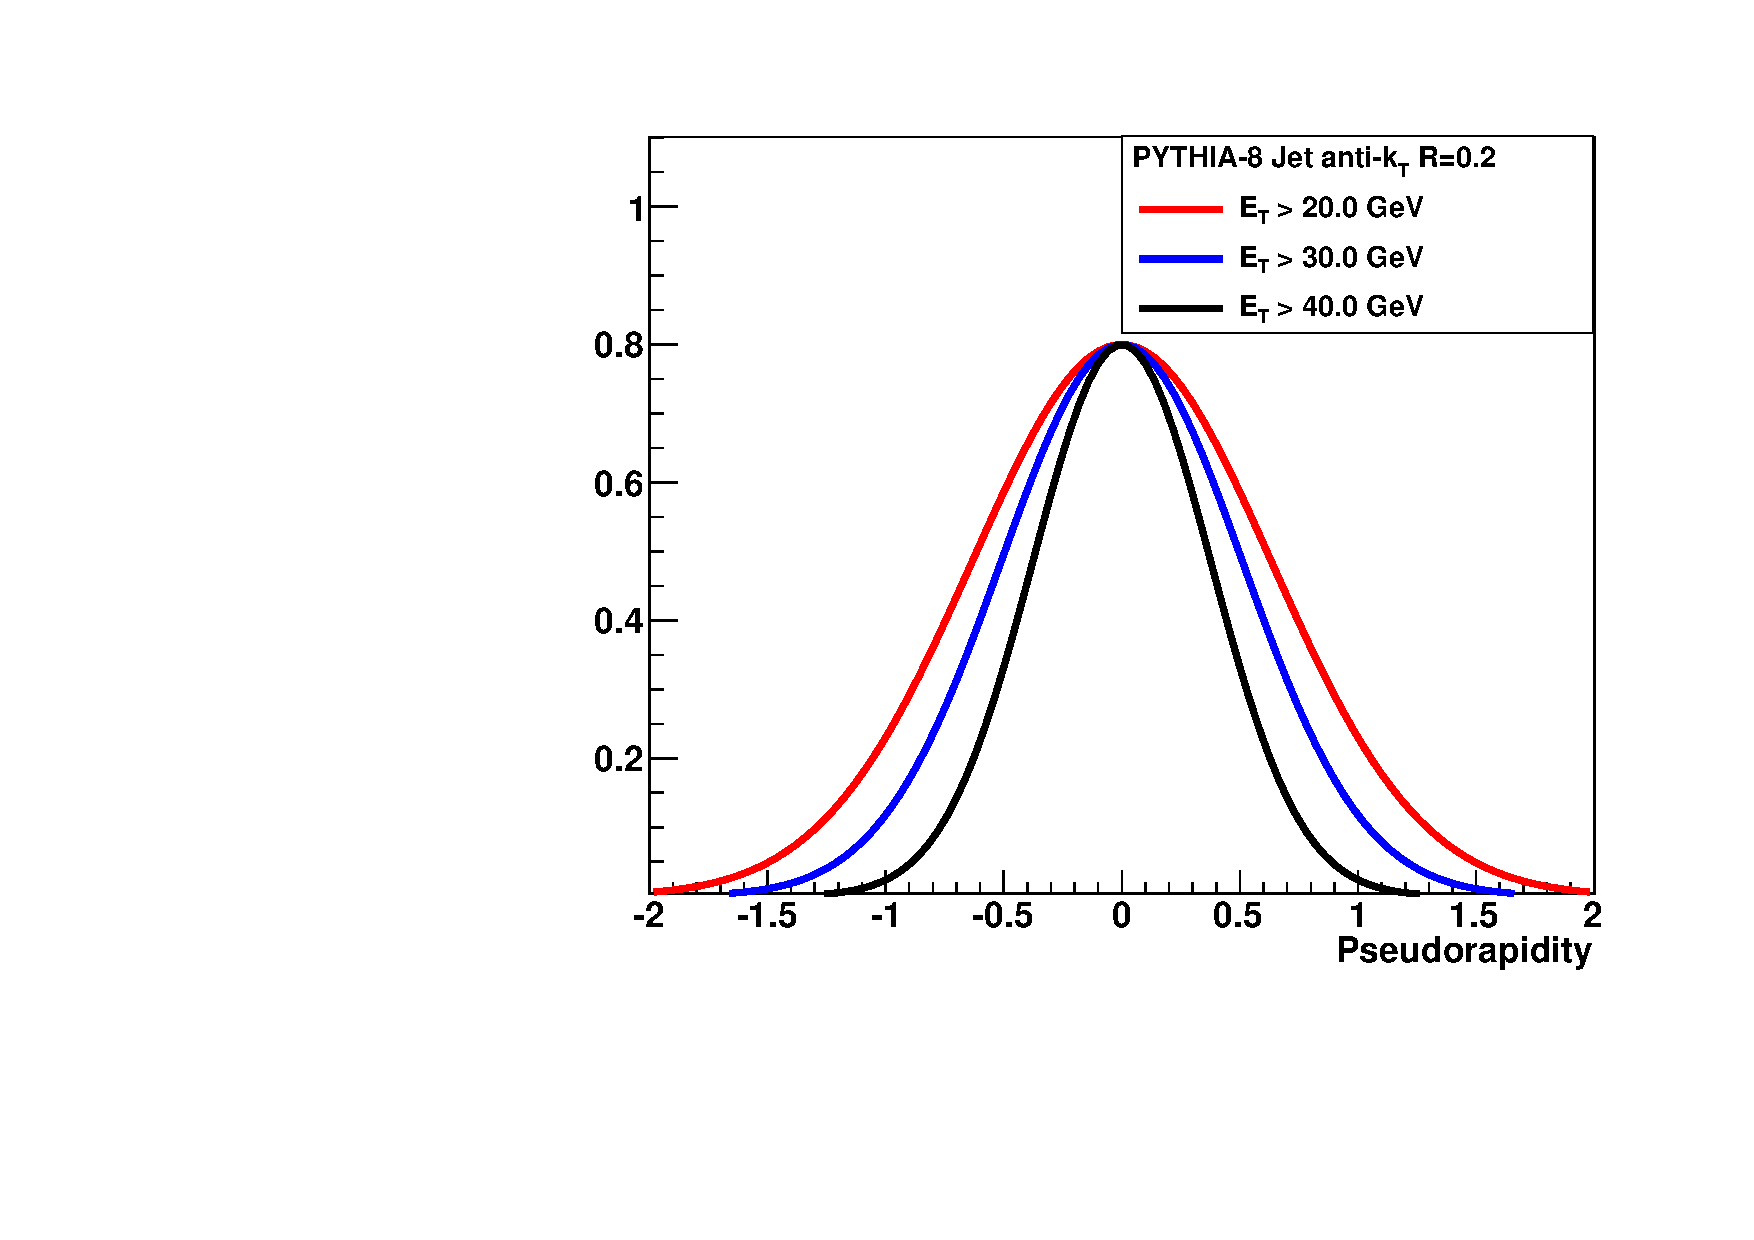
\includegraphics[trim = 2 2 2 2, clip, width=0.53\linewidth]{figs/figure_detectorrequirements_jetetadist}}
  \hfill
  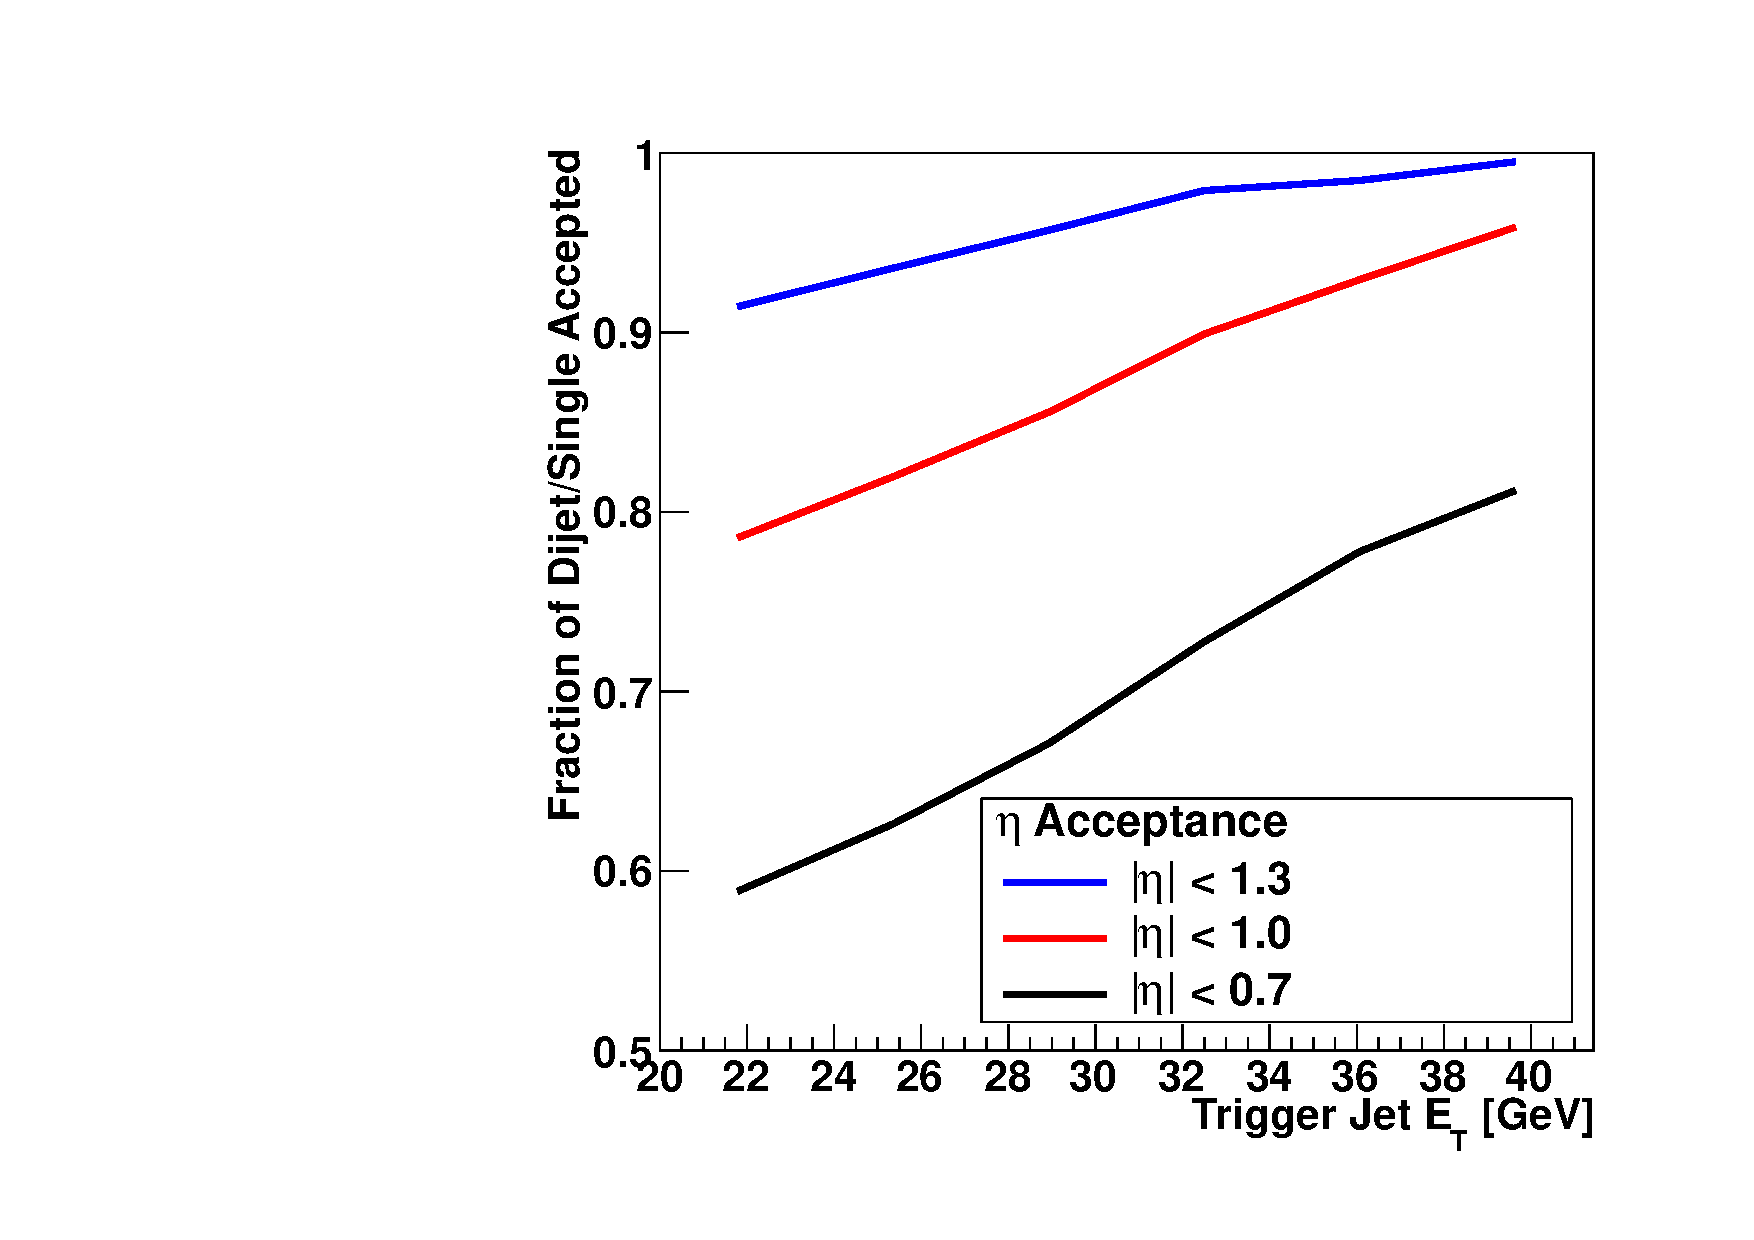
\includegraphics[trim = 2 2 2 2, clip, width=0.45\linewidth]{figs/figure_detectorrequirements_dijetaccept}
  \caption[Pseudorapidity distribution of \pythia jets reconstructed
  with the \fastjet anti-k$_{T}$ and the fraction of events in which
  the leading and subleading jet are in the specified
  acceptance]{\label{fig:pythia_dijet_accept}(Left) Pseudorapidity
    distribution of \pythia jets reconstructed with the \fastjet
    anti-k$_{T}$ and R=0.2 for different transverse energy selections.
    (Right) The fraction of \pythia events where the leading jet is
    accepted into a given pseudorapidity range where the opposite side
    jet is also within the acceptance.  Note that the current PHENIX
    acceptance of $|\eta|<0.35$ corresponds to a fraction below 30\%.}
 \end{center}
\end{figure}

